\documentclass[14pt]{extarticle}
\usepackage{amsmath}
\usepackage{amssymb}
\usepackage{tikz}
%\usetikzlibrary{calc}
\usetikzlibrary{trees}
\usepackage{hyperref}
\usepackage{graphicx}
\graphicspath{ {../../chap08/} }
\usepackage[top=0.75in, bottom=0.75in, left=0.75in, right=0.75in]{geometry}
\newcommand*{\Scale}[2][4]{\scalebox{#1}{\ensuremath{#2}}}%
\usepackage[shortlabels]{enumitem}
\usepackage[most]{tcolorbox}
\definecolor{bg}{RGB}{255,249,227}
% \usepackage{showframe}
\usepackage{caption}
\usepackage{fdsymbol}


\title{\vspace{-5ex}HANDOUT Math 208 Week 07}
\date{\vspace{-10ex}}
\usepackage{multicol}
\setlength{\columnsep}{.5cm}

\begin{document}
\maketitle		

\begin{tcolorbox}[enhanced jigsaw,colback=bg,boxrule=0pt,arc=0pt] 
	\textbf{Theorem: Assigning probability under the equally likely assumption}
	\begin{align*}
		P(E) = \frac{\text{number of elements in E}}{\text{number of elements in S}} = 
		\frac{n(E)}{n(S)}
	\end{align*}
\end{tcolorbox}

\textbf{Sample space for flipping a coin 3 times}: $n(S)= 2*2*2=8$ and 
$$S=\{HHH, HHT,HTH,THH,HTT,THT,TTH,TTT\}$$

\begin{enumerate}
	\item What is the probability that the first flip is heads or two flips are tails? What are the odds for? \vspace{1.5cm}
	\item What is the probability that the first flip is heads and two flips are tails? What are the odds against?
\end{enumerate}
\vspace{1.5cm}


\textbf{Sample space for rolling two dice}: $S$ is the set of all ordered pairs in the dice chart. $n(S) = 6*6 = 36$.

%\begin{figure}[h!]
%	\caption*{\textbf{Sample space for rolling two dice}: $S$ is the set of all ordered pairs in the figure. $n(S) = 6*6 = 36$.}
%	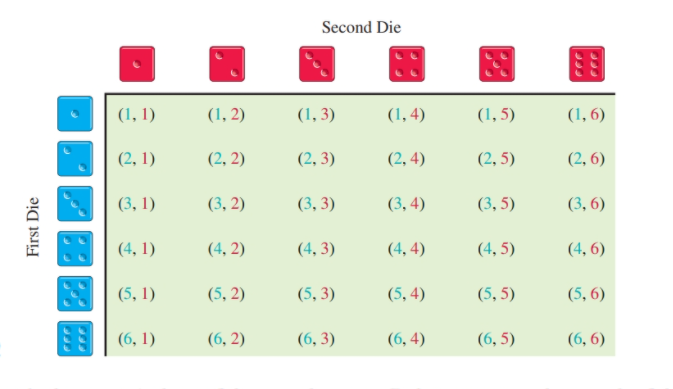
\includegraphics[width=.8\linewidth]{8-1-5}
%\end{figure}

\begin{multicols}{2}
\begin{enumerate}
	\item $P((2,2))=$ \vspace{1.2cm}
	\item $P($first die is 4$)=$ \vspace{1.2cm}
	\item $P(sum=7)=$ \vspace{1.2cm}
	\item $P($sum is prime$)=$ \vspace{1.2cm}
	\item $P($sum is 7 and prime$)=$ \vfill\null\columnbreak
	\item $P($sum is 7 or prime$)=$ \vspace{1.2cm}
	\item $P($sum $< 4$ or sum $\geq 11)=$\vspace{1.2cm}
	\item $P($sum $\geq 4$ and sum $< 11)=$\vspace{1.2cm}
	\item $P($first die is 4 $\cap$ sum is prime $)=$\vspace{1.2cm}
	\item $P($first die is 4 $\cup$ sum is prime $)=$\vfill\null
\end{enumerate}
\end{multicols}
\vspace{1.2cm}
\begin{multicols}{2} [What are the odds in favor?]
	\begin{enumerate}
		\item $P((2,2))=$ \vspace{1.2cm}
		\item $P($first die is 4$)=$ \vspace{1.2cm}
		\item $P(sum=7)=$ \vspace{1.2cm}
		\item $P($sum is prime$)=$
	\end{enumerate}
\end{multicols}
\vspace{1.2cm}
\begin{multicols}{2} [What are the odds against?]
	\begin{enumerate}
		\item $P($sum is 7 and prime$)=$ \vspace{1.2cm} 
		\item $P($sum is 7 or prime$)=$ \vspace{1.2cm}
		\item $P($sum $< 4$ or sum $\geq 11)=$\vspace{1.2cm}
		\item $P($sum $\geq 4$ and sum $< 11)=$\vspace{1.2cm}
	\end{enumerate}
\end{multicols}
\vspace{1.2cm}

\textbf{Sample space for a deck of 52 cards}: $S$ is the set of all possible drawn hands. When working with cards, the order of the draw typically does NOT matter. For a 5 card draw, $n(S)=_{52}C_5 = 2598960$. Probabilities of cards becomes much more complex than dice.

%\begin{figure}[h!]
%	\caption*{\textbf{Sample space for a deck of 52 cards}: $S$ is the set of all possible drawn hands. When working with cards, the order of the draw typically does NOT matter. For a 5 card draw, if the order of the draw does not matter, $n(S)=_{52}C_5 = 2598960$.}
%	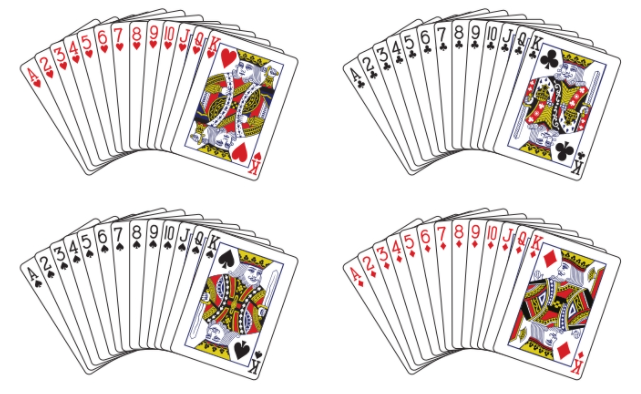
\includegraphics[width=.8\linewidth]{cards}
%\end{figure}
%Working with the probabilities of cards is much more complex than dice.
%$\color{red}\clubsuit \diamondsuit \spadesuit \varheartsuit$
\begin{multicols}{2}[Find the probability from the draw of a single card.]
	\begin{enumerate}
		\item $P($A$\color{red}\heartsuit$$)=$ \vspace{1.3cm}
		\item $P($K$)=$ \vspace{1.3cm}
		\item $P($$\color{red}\heartsuit$$)=$ \vspace{1.3cm}
		\item $P($$\clubsuit$ or $\spadesuit$$)=$ \vfill\null\columnbreak
		\item $P($10 or $\color{red}\heartsuit$$)=$ \vspace{1.3cm}
		\item $P($not(10 or $\clubsuit$)$)=$ \vspace{1.3cm}
		\item $P($face card$)=$ \vspace{1.3cm}
		\item $P($not face card$)=$ \vfill\null
	\end{enumerate}
\end{multicols}
\vspace{1cm}
\begin{multicols}{2}[Find the probability from the draw of five cards.]
	\begin{enumerate}
		\item $P($A$\color{red}\heartsuit$$)=$ \vspace{1.6cm}
		\item $P($exactly one $\color{red}\heartsuit$$)=$ \vspace{1.6cm}
		\item $P($at least one $\color{red}\heartsuit$$)=$\vspace{1.6cm}
		\item $P($all $\color{red}\heartsuit$$)=$ \vfill\null\columnbreak
		\item $P($10JQKA$\color{red}\heartsuit$$)=$ \vspace{1.6cm}
		\item $P($royal flush$)=$ \vspace{1.6cm}
		\item $P($four Aces$)=$ \vspace{1.6cm}
		\item $P($four of a kind$)=$ \vfill\null
	\end{enumerate}
\end{multicols}

\begin{tcolorbox}[enhanced jigsaw,colback=bg,boxrule=0pt,arc=0pt] 
	\textbf{Conditional Probability}
	\begin{align*}
		P(A|B)&=\frac{n(A\cap B)}{n( B)} =  \frac{P(A\cap B)}{P(B)}
	\end{align*}
	and
	\begin{align*}
		P(A\cap B) = P(A)P(B|A) = P(B)P(A|B)
	\end{align*}
\end{tcolorbox}

\textbf{For rolling two dice}
\begin{enumerate}
	\item $P($first die is 4 $\mid$ second die is 4$)=$ \vspace{1.2cm}
	\item $P($sum=7 $\mid$ first die is 4$)=$ \vspace{1.2cm}
	\item $P($sum is prime $\mid$ sum is 7$)=$ \vspace{1.2cm}
	\item $P($sum $\leq 7 \mid$ sum is prime$)=$ \vspace{1.2cm}
\end{enumerate}
\vspace{1.2cm}

\begin{multicols}{2}[Find the probability from the draw of five cards.]
	\begin{enumerate}
		\item $P($A$\mid\clubsuit$) \vspace{1.6cm}
		\item $P($exactly one $\clubsuit$$\mid$first is $\clubsuit$) \vspace{1.6cm}
		\item $P($at least one $\clubsuit$$\mid$first is $\clubsuit$) \vfill\null\columnbreak
		\item $P($all $\clubsuit$$\mid$first is $\clubsuit$) \vspace{1.6cm}
		\item $P($face card$\mid\clubsuit$) \vspace{1.6cm}
		\item $P($four Aces$\mid$four of a kind) \vfill\null
	\end{enumerate}
\end{multicols}
\vspace{1cm}


\section*{Probability Applications}
\begin{enumerate}
	\item In a family with 2 children, excluding multiple births, what is the probability of having 2 girls? Assume that a girl is as likely as a boy at each birth.
	\vspace{2cm}

	\item \textbf{Personnel selection}. Suppose that 6 female and 5 male applicants have been successfully screened for 5 positions. If the 5 positions are filled at random from the 11 finalists, what is the probability of selecting 
	\begin{enumerate}
		\item 3 females and 2 males?
		\vspace{2cm}
		\item 4 females and 1 male?
		\vspace{2cm}
		\item 5 females?
		\vspace{2cm}
		\item At least 4 females?
		\vspace{2cm}
	\end{enumerate}
	
	\item \textbf{Market research}. From a survey involving 1,000 university students, a market research company found that 750 students owned laptops, 450 owned cars, and 350 owned cars and laptops.
	\begin{multicols}{3}[Empirical probabilities]
			P(laptop) = \vfill\null\columnbreak
			P(car) = \vfill\null\columnbreak
			P(car and laptop) = \vfill\null
	\end{multicols}
	If a university student is selected at random, what is the (empirical) probability that:
	\begin{enumerate}
		\item The student owns either a car or a laptop?
		\vspace{2cm}
		\item The student owns neither a car nor a laptop?
		\vspace{2cm}
		\item The student does not own a car?
		\vspace{2cm}
		\item The student owns a car but not a laptop?
		\vspace{2cm}
	\end{enumerate}
\end{enumerate}




\noindent\rule{\textwidth}{1pt}
{\footnotesize Copyright (C) 2021 Garold Dalton --- Released under GNU General Public License v3.0}


\cleardoublepage


\end{document}
